\begin{figure*}[t]
  \centering
  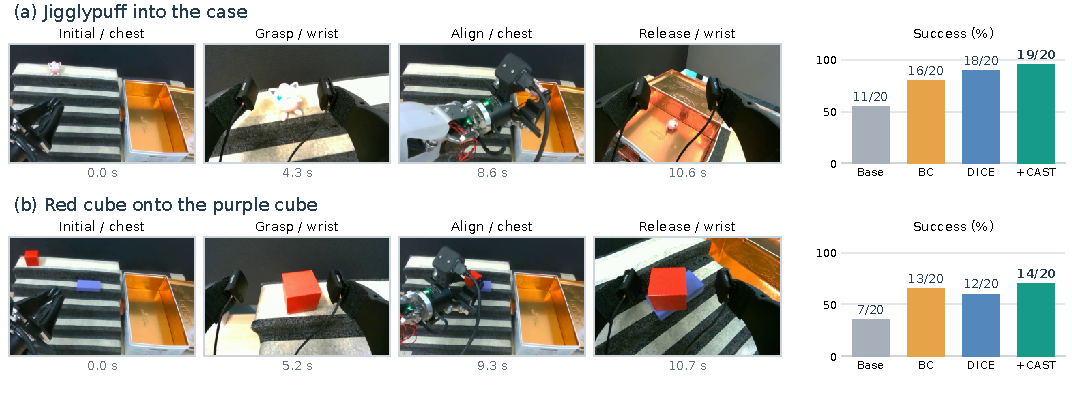
\includegraphics[width=\textwidth]{figures/real_robot_tasks.pdf}
  \caption{OpenArm task demonstrations and autonomous evaluation results.
  Each row shows initial, grasp,
  align, and release stages, using chest, left-wrist, chest, and left-wrist
  views, respectively. These are
  successful \emph{teleoperated demonstrations},
  not autonomous evaluations of the compared methods. Times are nominal
  video times at 15 fps, using the source stage frame indices.
  A common background crop is used throughout. The fifth panel reports
  autonomous success over 20 trials per method for that row's task, with
  successes/trials above the bars and a shared percentage scale. Base is
  the pretrained FM policy; BC is success-only refinement; DICE and +CAST
  are DICE-RL and DICE-RL + CAST. Bold counts mark the highest observed
  success. Jigglypuff poses are randomized on the stairs.}
  \label{fig:real-robot}
\end{figure*}
